\section{Lektion 06-03-2018}

\begin{enumerate}
	\item Quality Software - Object Oriented Design and DSP (C++)
	\item Design Patterns
	\item 3-Layered Architecture
	\item DSP Design Framework
\end{enumerate}

\subsection{Quality Software}
\subsubsection{Characterization}
\begin{itemize}
	\item Easy to maintain and expand because of its clear architecture and flexibility.
	\item Have a high degree of reuse - \textbf{low coupling} and h\textbf{igh cohesion}, modularization.
	\item Easy to understand both high and low level of	abstraction – \textbf{simplicity}.
	\item Have easily recognizable \textbf{design patterns} - provide understanding.
	\item Other programmers will not be afraid working on
	it - \textbf{understandable}.
\end{itemize}
\newpage
\subsection{Object Oriented Design C++}
\begin{itemize}
	\item Classes - Abstract Data typing - Incapsulation
	\item Abstract base classes - Interfaces
	\item Virtual member functions - Polymorphism
	\item Operator overloading
	\item Inheritance
	\item Templates
\end{itemize}

\subsubsection{Hard and soft real-time systems}
A real-time system must react to stimuli from the operator or other devices within time intervals dictated by its environments. 
A deadline is the instant at which a result must be performed. 
A system with at least one hard deadline is called a hard real-time system else a soft real-time system.

\begin{itemize}
	\item \textbf{Soft deadline}
	\begin{itemize}
		\item System can miss some deadlines, but eventually performance will degrade if too many are missed. The result is accepted to be ready after the deadline.
	\end{itemize}
	\item \textbf{Hard deadline}
	\begin{itemize}
		\item System must absolutely hit every deadline. Missing a deadline constitutes a system failure.
	\end{itemize}
\end{itemize}

\subsubsection{C++ features}
\begin{itemize}
	\item Many C++ features have no performance cost.
	\begin{itemize}
		\item Namespaces, overloaded functions, inheritance. 
	\end{itemize}
	\item Avoid dynamic allocation using new and delete – use static allocations
if \textbf{hard deadline}.
	\item Same goes for minimizing use of virtual functions and keeping basic data types in structures.
\end{itemize}

\subsection{Design Patterns}
\begin{itemize}
	\item Describes a problem that occurs again and	again.
	\item Provides a general solution to the problem.
	\item The basis for the implementation of an object-oriented language.
	\item Improves reuse of design.
	\item Improve understanding and communication of a design.
	\item A design pattern consists of 4 elements:
	\begin{itemize}
		\item Name of the design pattern.
		\item Problem description.
		\item Solution and its objects (relationships, responsibility and cooperation).
		\item Impact of solution (trade-offs and cost/benefits).
	\end{itemize}
\end{itemize}

\subsubsection{Types}
\begin{itemize}
	\item Creational Patterns
	\begin{itemize}
		\item Responsible for creating objects
	\end{itemize} 
	\item Structural Patterns
	\begin{itemize}
		\item Describes the composition of classes and objects
	\end{itemize}
	\item Behavioral Patterns
	\begin{itemize}
		\item Describes the interaction between classes and objects
		and allocation of responsibilities
	\end{itemize}
\end{itemize}

\paragraph{Composite} combines items for tree structures to represent part-whole hierarchies. It lets clients treat primitive and composite objects in the same way.\\

\noindent Use the composite pattern when representating a "part-whole" structure. When no distinction should be drawn (from client side) between the individual and composite objects and all objects in the structure (primitive and composite) must be handled in a consistent manner.
\newpage\begin{itemize}
	\item \textbf{Pros}
	\begin{itemize}
		\item Primitive objects can be combined into complex objects.
		\item Makes the client simple (avoid case statements).
		\item Easy to add new types of objects; no affect on client's code
	\end{itemize}
	\item \textbf{Cons}
	\begin{itemize}
		\item Can make the code too general.
		\item \mintinline{c}{Add()} and \mintinline{c}{Remove()} in primitive objects	does not make sense.
	\end{itemize}
\end{itemize}
\begin{figure} [H]
	\centering
	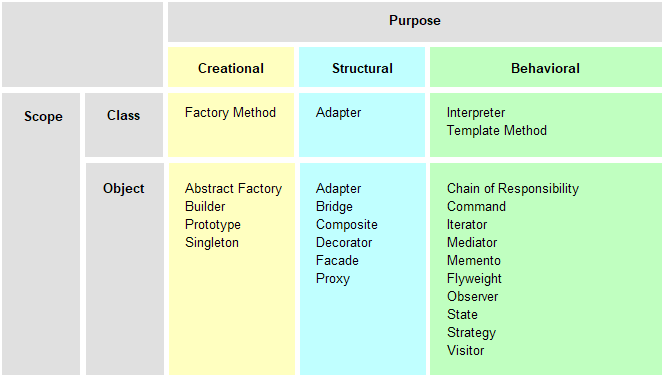
\includegraphics[width=\linewidth]{graphics/23.png}
	\caption{Gof Design Patterns, \href{https://circle.visual-paradigm.com/catalog/}{Visual Paradigm Community Circle}}
	\label{fig:23}
\end{figure}

\newpage \subsection{3-Layered Architecture}

\begin{itemize}
	\item Change in presentation layer (boundary) makes no changes in the
	other layers. (perhaps in control)
	\item Change in control layer (control) may	lead to changes in the boundary layer.
	\item Changes in the domain layer (domain) 	can cause changes in all layers.
\end{itemize}

\begin{figure} [H]
	\centering
	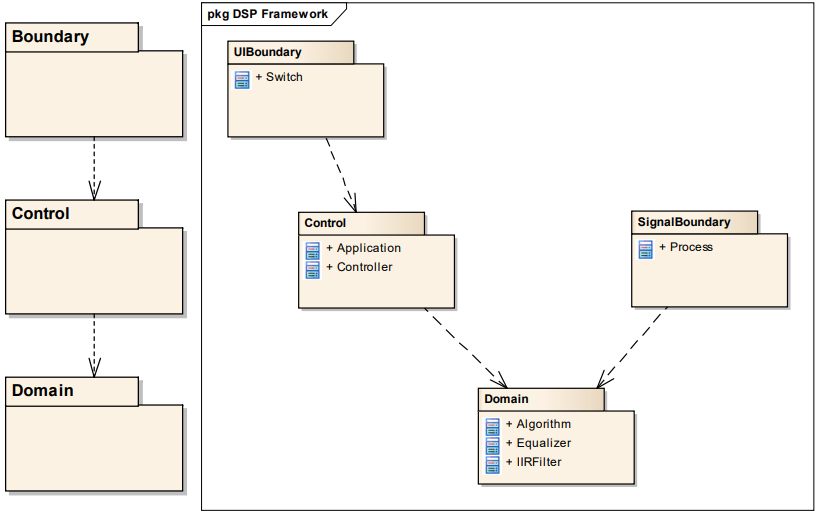
\includegraphics[width=\linewidth]{graphics/22.png}
	\caption{DSP Layered Design.}
	\label{fig:22}
\end{figure}


\subsection{DSP Design Framework}
\begin{itemize}
	\item The framework provides a \textbf{clear architecture with flexibility} being able to change UI or adding new	algorithms.
	\item The framework has a degree of reuse with \textbf{low coupling} and \textbf{high cohesion}, realized with a layered architecture and classes with well defined responsibility.
	\item Efficient design - use of \textbf{static object instantiation}.
	\item The framework uses recognizable \textbf{design patterns} – build on the 3 layer model, composite and pipes and filters patterns
	\item Hopefully \textbf{understandable} for other programmers!
\end{itemize}


